\documentclass[12pt]{article}
 
\usepackage[margin=1in]{geometry} 
\usepackage{amsmath,amsthm,amssymb}
\usepackage{gensymb}
\usepackage{hyperref}
\usepackage{graphicx}
 

\begin{document}

\date{\today}
\title{Procedure for analyzing T. Brown HST data from 2010 and 2012 with Dolphot}
\author{Sean Terry \& Ishaan Gandhi} 
 
\maketitle

\noindent {\footnotesize Keywords: \\
\\
``CMD" = Color-Magnitude Diagram \\
``DM" = Dolphot Manual \\
``DS9" = SAOImage DS9 Program  \\
``HST" = Hubble Space Telescope \\
``img2xym.F" = Image to x, y, magnitude (Fortran program) \\
``IR" = Infrared (filters) \\
``LF" = Luminosity Function \\
``MAST" = Mikulski Archive for Space Telescopes \\
``PM" = Proper Motion \\
``WFC3" = Wide Field Camera 3 \\
``WFC3M" = Wide Field Camera 3 Manual \\
``UVIS" = Ultraviolet and Visible (filters) \\
}

\begin{section}{Preliminary}
Programs needed: \\
\textbf{Dolphot} -- Dolphin Photometry (author: Andrew Dolphin, Raytheon Company) \\
\textbf{DS9} -- Image Visualization Package (author: Smithsonian Astrophysical Observatory) \\
\textbf{Python}


\end{section}
\begin{section}{Data}
This section describes retrieving the relevant data and preparing it for analysis. All of the images were taken using the HST WFC3, of a portion of sky located near the galactic center. Images were taken June 27, 2010 and June 27, 2012, approximately two calendar years apart.
\begin{subsection}{MAST}
The HST data to be downloaded from the MAST archive is as follows: \\
\begin{itemize}
\item F555W/F814W/F160W/F110W filter data from WFC3 of the ``Stanek" field (Proposal ID: 11664) This is 2010 data.
\item F814W filter data from WFC3 of the ``Stanek" field (Proposal ID: 12666) This is 2012 data.
\end{itemize}
\end{subsection}

\begin{subsection}{Prep Data}
Once files are downloaded, place them in separate (by filter) working directories (don't forget to create backups of all files as Dolphot will actively alter them during processing!) Now move only the ``\texttt{*\_flc.fits}" files into a separate (by filter again) working directory. 
\end{subsection}
\end{section}

\begin{section}{Running Dolphot}
Dolphot will be run from the terminal within the current working directory. Most of the steps listed here will refer to the DM or the WFC3M. At this point, creating/selecting a reference image is not necessary for our analysis. The steps for analysis are as follows: \\
\begin{subsection}{F110W and F160W IR Images}
\begin{itemize}
\item Run `wfc3mask' (ref. WFC3M)
\item Run `calcsky' (ref. WFC3M)
\item Run `dolphot' (ref. WFC3M)
\end{itemize}
\end{subsection}

\begin{subsection}{F814W and F555W UVIS Images}
\begin{itemize}
\item Run `wfc3mask' (ref. WFC3M)
\item Run `splitgroups' (ref. WFC3M)
\item Run `calcsky' (ref. WFC3M)
\item Run `dolphot' (ref. WFC3M)
\end{itemize}
\end{subsection}
There are several outputs from the routine; most importantly is the main photometry list (no file extension) and the `.columns' file which describes each column printed out in the photometry list. \\
\\
A small Python script can be written to condense this master photometry list down to an array with just the relevant quantities desired (x-position, y-position, object type, instrumental magnitude, magnitude uncertainty, etc). Cuts can also be made on the array to reject object types not listed as `star' (ref. DM and WFC3M).

\end{section}

\begin{section}{Color-Magnitude Diagrams}
CMD's (F110W - F160W vs. F160W, and F555W - F814W vs. F814W) can be generated from the Dolphot master photometry lists by simply calculating the color (difference in instrumental magnitude between F110W/F160W and F555W/F814W respectively) and plotting it against the instrumental magnitude column in the various filters. Calculating an example CMD from F555W and F814W would be something like; \\
\\
Column 16 (F555W magnitude) - Column 29 (F814W magnitude), print to new column (call it `color'). Then just plot `color' column versus column 16 or 29. Color is x-axis, magnitude is y-axis. Here is one CMD that has been created thus far: \\
{\center{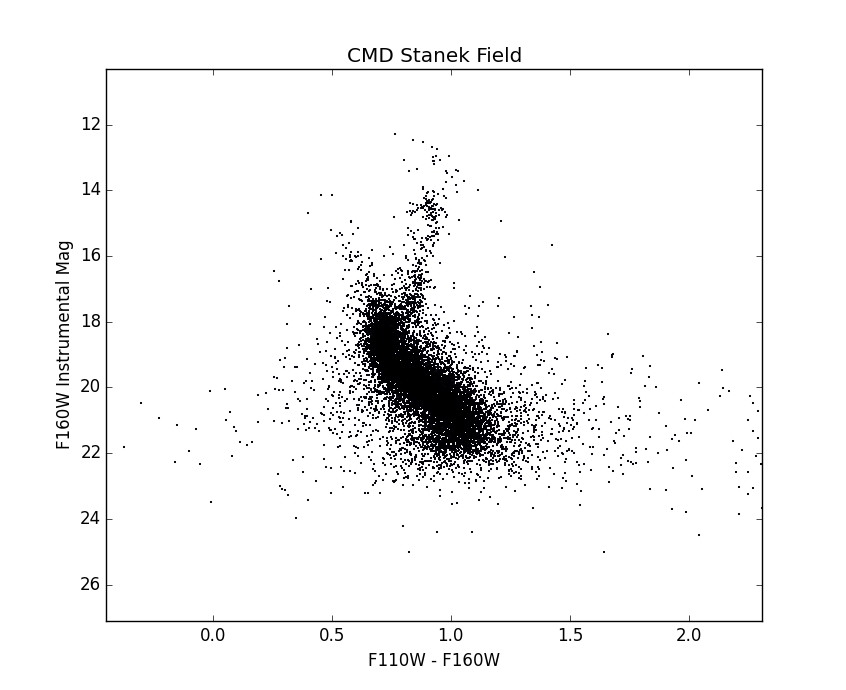
\includegraphics[scale=0.70]{stanekcmd.png}}} \\
\textbf{IMPORTANT:} This CMD includes both bulge stars AND foreground disk stars. Our aim for this part of the project is to generate disk-decontaminated CMD's that are composed primarily of only bulge stars. The most efficient way to do this is by matching and rejecting stars by their proper motions, which we explain in section 5.

\end{section}

\begin{section}{Proper Motions and CMD-Cleaning}

The procedure for calculating the stellar PM's and cleaning the CMD's is quite tedious. The stars in the F814W images between 2010 and 2012 only move about one-half of a pixel in the x-direction and one-third of a pixel in the y-direction. A complicating factor is a systematic `jitter' that is present between the images. This jitter is due to uncertainty in the WCS coordinates listed from the telescope itself. The magnitude of the jitter is about three pixels in the x-direction and one pixel in the y-direction; much larger than the actual proper motions of the stars themselves. The solution for correcting this jitter is currently being worked on. \\
\\ 
A few ideas to resolve this issue are:
\begin{itemize}
\item Manually determine the precise jitter value in x and y and correct for this either in DS9 or another image matching program.
\item Using an `Alignment' value that Dolphot outputs, determine the stellar shifts and somehow back-out the jitter and/or PM values.
\item The `wfc3distort' command in Dolphot might be useful for manually matching the two images precisely in order to get PM's for individual stars.
\item Emailed Jay Anderson about possibly using his routine \textbf{img2xym.F} for calculating VERY precise proper motion measurements (this does not solve the `jitter' seen between the images.
\end{itemize}



\end{section}






 
\end{document}